\section{Methodology}
\label{sec:methodology}
We treat each relevant consumer-item as an individual object and shape them into weekly time series data
based on historical transactions. In this setup, target value at each time step (week) takes a binary input, 1/0 
(purchased/non purchased). \emph{Relevancy} of the consumer-item is defined by items transacted by consumer during training 
time window. \emph{Postive samples} (purchased/1) are weeks where consumer did transact for an item, whereas 
\emph{Negative samples} (non purchased/0) are the weeks where the consumer did not buy that item.
We apply sliding windows testing routine for generating
out of time results. The time series is split into 4 parts - train, validation, 
test1, and test2 as shown in Table \ref{tab:datasplit}. All our models are built in a multi-object 
fashion, which allows the gradient movement to happen across all consumer-item combinations split in batches. This enables 
cross-learning to happen across consumers/items. We then perform Feature Engineering over data splits to generate
modelling features. Below are some of the feature groups we perform our experiments with:
\begin{itemize}
\item {\bf Datetime:} We use transactional metrics at various temporal cuts like week, month, etc.
Datetime related features capturing seasonality and trend are also generated.
\item {\bf Consumer-Item Profile:} We use transactional metrics at different granularities like consumer, item,
consumer-item, department and aisle. We also create features like Time since first order, 
Time since last order, time gap between orders, Reorder rates, Reorder frequency, 
Streak - user purchased the item in a row, Average position in the cart, Total number of orders.
\item {\bf Consumer-Item-Time Profile:} We use transactional metrics at the intersection of consumer, item and time.
We generate interactions capturing consumer behaviour towards items at a given time.
\item {\bf Lagged Offsets:} We use statistical rolling operations like mean, median, quantiles, variance, 
kurtosis and skewness over temporal regressors for different lag periods to generate offsets.
\end{itemize}
The model we need to build, thus, should learn to identify similarly behaving time series across latent
parameters, and take into account consumer and item variations in comparing different time series. A row 
in time series is represented by
  \begin{equation}
    \begin{array}{l}
      y\textsubscript{cit}  = f(i\textsubscript{t}, c\textsubscript{t},..,c\textsubscript{t-n}, ic\textsubscript{t}
      ,..,ic\textsubscript{t-n}, d\textsubscript{t},..,d\textsubscript{t-n})
    \end{array}
    \label{eqn:fx}
  \end{equation}
where y\textsubscript{cit} is purchase prediction for consumer 'c' for item ’i’ at time ’t’. 
i\textsubscript{t} denotes attributes of item ’i’ like category, department, brand, color, size, etc at time 't'. 
c\textsubscript{t} denotes attributes of consumer 'c' like age, sex and transactional attributes at time 't'. 
ic\textsubscript{t} denotes transactional attributes of consumer 'c'  towards item 'i' at time 't'. 
d\textsubscript{t} is derived from datetime to capture trend and seasonality at time 't'. 
'n' is the number of time lags.
\begin{table}[t]
\caption{Modelling data splits}
\vspace{0.1 in}
\centering
\resizebox{3.3in}{!}
{%
\begin{tabular}{|c|c|c|c|}
\hline
{\bf Data Split} & {\bf Specifications} & {\bf Consumer-Item combinations} & {\bf Max Time-Series length} \\  
\hline\hline
Train  		&  Model training &  50,872 &  46 weeks \\ \hline
Validation	  		&  HyperParameter Optimization &  50,888 &  2 weeks \\ \hline
Test1  		&  Stacked Generalization, F\textsubscript{1}-Maximization & 50,899 &  2 weeks\\ \hline
Test2	  		&  Reporting Accuracy Metrics & 50,910 &  2 weeks\\
\hline
\end{tabular}
}
\label{tab:datasplit}
\end{table}
\subsection{Loss Function}
Since we are solving Binary classification problem, we believe that Binary Cross-Entropy should be the most appropriate 
loss function for training the models. We use the below formula to calculate Binary Cross-Entropy:
  \begin{equation}
      \begin{array}{l}
        H\textsubscript{p} = - \frac{1}{N}$$\sum_{i=1}^{N}y.log(p(y))+
        (1- y).log(1-p(y))
      \end{array}
    \label{eqn:logloss}
  \end{equation}
here H\textsubscript{p} represents computed loss, y is the target value (label), and p(y) 
is the predicted probability against the target. The BCELoss takes non-negative values. We can infer 
from Equation \ref{eqn:logloss} that Lower the BCELoss, better the Accuracy.
\subsection{Model Architectures}
As mentioned earlier in this section, traditional machine learning models are not really a suitable choice for modelling \emph{f} 
(Equation \ref{eqn:fx}) due to non-linear interaction of the features. Hence, we work with
tree based models like RandomForest, Xgboost \cite{chen2016xgboost} 
to Deep learning models like Multi Layer Perceptron (MLP), Long Short 
Term Memory (LSTM) and Temporal Convolutional Networks (TCN). Architectures of MLP, LSTM, TCN \cite{lea2016temporal} 
and TCN-LSTM \cite{karim2017lstm} models are shown in Figure \ref{fig:MLP}, Figure \ref{fig:LSTM}, Figure \ref{fig:TCN}
and Figure \ref{fig:TCN-LSTM} respectively. We briefly describe the architectures below.
\begin{itemize}
\item {\bf Entity Embeddings + Multi Layer Perceptron:} MLP (Figure \ref{fig:MLP}) is the simplest form of deep neural networks 
and was originally proposed in \cite{wang2017time}. The architecture contains 
three hidden layers fully connected to the output of its previous layer. The final layer 
is the sigmoid layer which generates the probability. One disadvantage of MLP is that since the input time 
series is fully connected to the first hidden layer, the temporal information in a time series is lost \cite{fawaz2019deep1}.
\item {\bf Entity Embeddings + Long Short Term Memory:} LSTM (Figure \ref{fig:LSTM}) is an
architecture comprising of 2 LSTM layers combined with entity embeddings. This combination flows into 
3 fully connected ReLU based layers yielding to dense layer which has sigmoid activation.
\item {\bf Entity Embeddings + Temporal Convolutional Network:} TCN (Figure \ref{fig:TCN}), originally
proposed in \cite{lea2016temporal} , is considered a competitive architecture yielding the best results when evaluated over 
our experimental dataset. This network comprises of 3 dilated Convolutional networks combined with entity embeddings.
Similar to LSTM, this architecture, after convolving and concatenating, it flows into 
3 fully connected ReLU based layers yielding to dense layer which has sigmoid activation.
\item {\bf Entity Embeddings + Long Short Term Memory-Temporal Convolutional Network:} TCN-LSTM (Figure \ref{fig:TCN-LSTM})
inherits the properties of LSTM and TCN in a fully connected network.
\end{itemize}
From data classification, Figure \ref{fig:dnndata}, we can see that data was sub-divided 4 groups:
\begin{itemize}
\item {\bf Static Categorical:} These are categorical features that do not vary with time. This includes consumer
attributes like sex, marital status and location along with different item attributes like category, department and brand.
\item {\bf Temporal Categorical:} These are categorical features that vary with time. It includes all the datetime 
related features like week, month of year, etc.
\item {\bf Static Continuous:} These features are static but Continuous. This includes certain consumer attributes like
age and weight, item attributes like size, and certain derived features like target encoded features.
\item {\bf Temporal Continuous:} These are time varying Continuous features. All consumer and item related
traditional attributes like number of orders, add to cart order, etc. falls under this bucket.
\end{itemize}
As mentioned earlier in this section, in all the above described neural network architectures, we learn the embeddings \cite{guo2016entity} of the 
categorical features during training phase. We embed these attributes in order to compress their representations 
while preserving salient features, and capture mutual similarities and differences.
  \begin{figure}[t]
    \centering 
    \caption{Data classification for DNN Architectures} 
    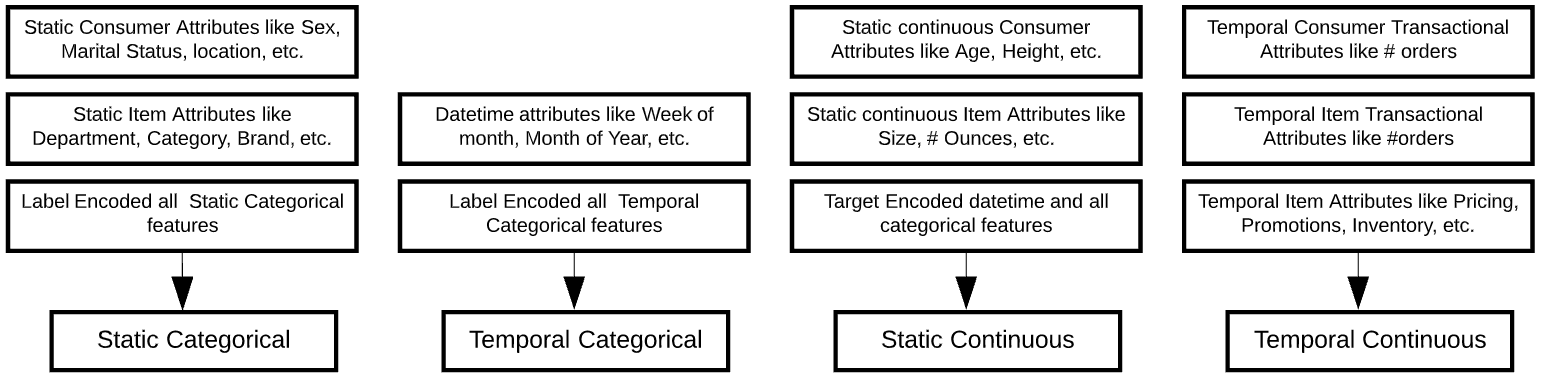
\includegraphics[width=3.3in]{img/dnndata.png} 
    \label{fig:dnndata} 
  \end{figure}
  \begin{figure}[t]
    \centering 
    \caption{Multi Layer Perceptron (MLP)} 
    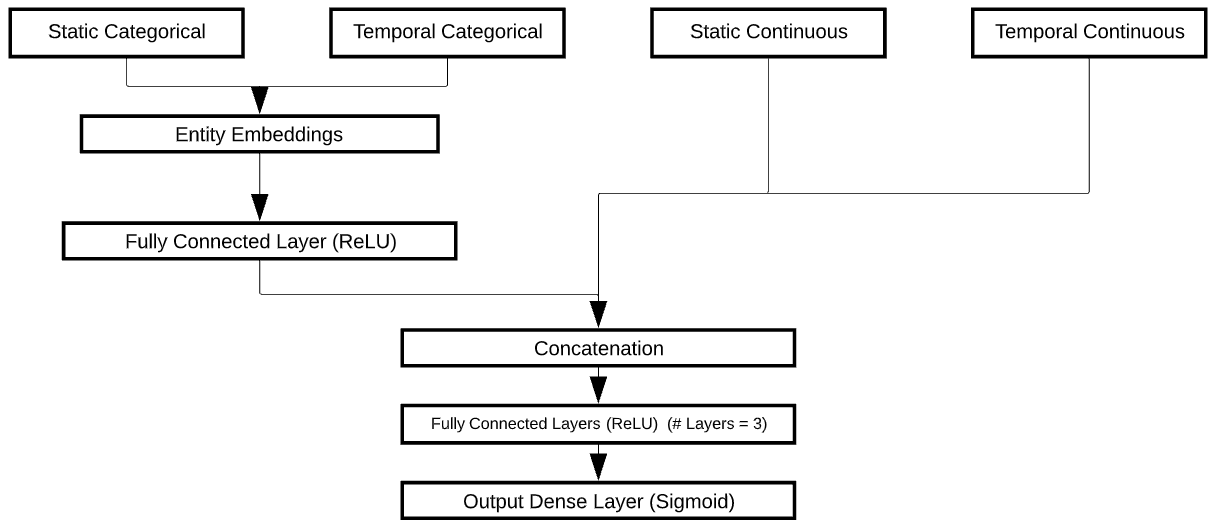
\includegraphics[width=3.3in]{img/MLP.png} 
    \label{fig:MLP} 
  \end{figure}
  \begin{figure}[t]
    \centering 
    \caption{Long Short Term Memory (LSTM)} 
    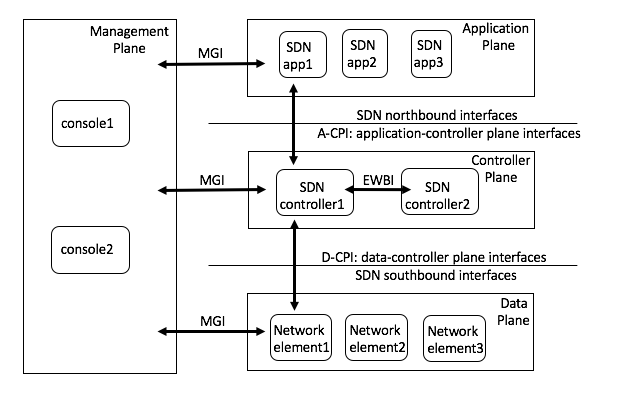
\includegraphics[width=3.3in]{img/LSTM.png} 
    \label{fig:LSTM} 
  \end{figure}
  \begin{figure}[t]
    \centering 
    \caption{Temporal Convolutional Network (TCN)} 
    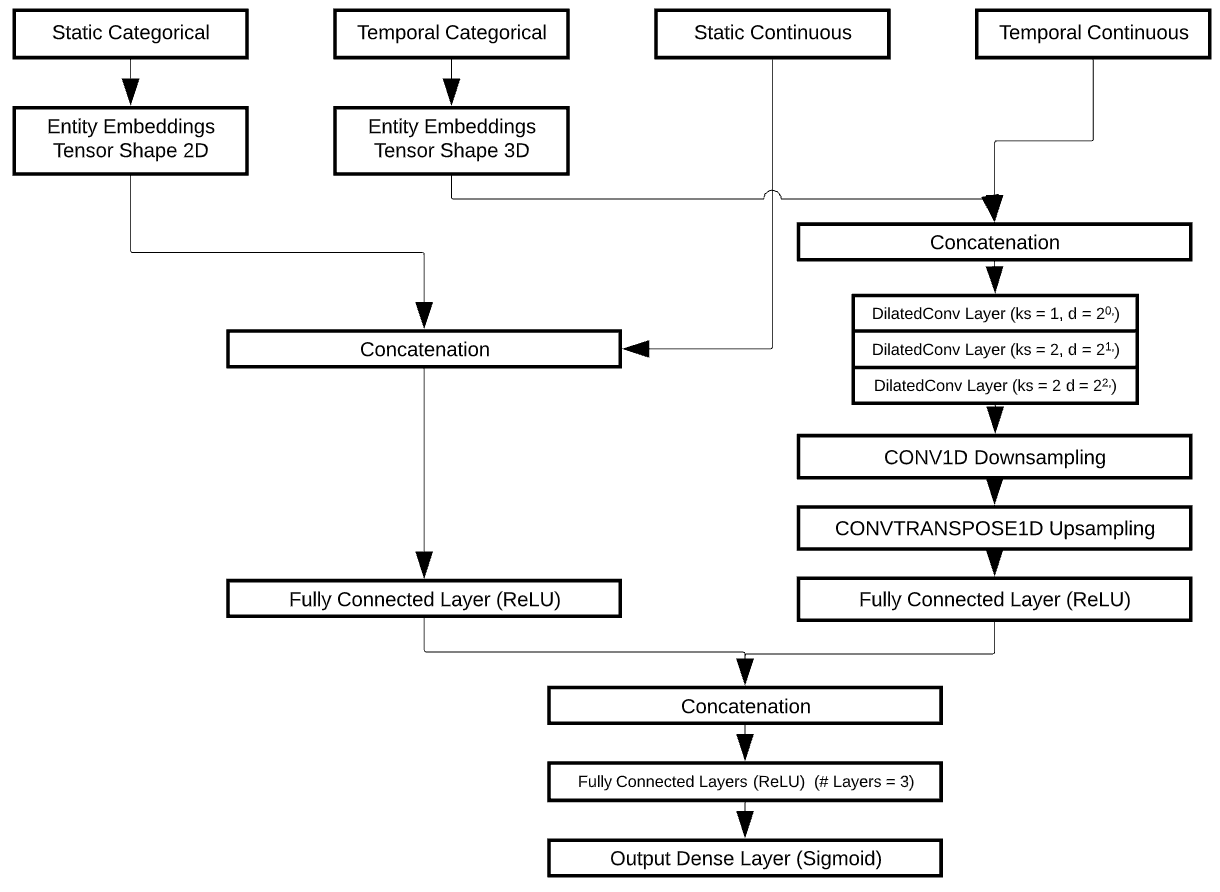
\includegraphics[width=3.3in]{img/TCN.png} 
    \label{fig:TCN} 
  \end{figure}
  \begin{figure}[t]
    \centering 
    \caption{TCN-LSTM} 
    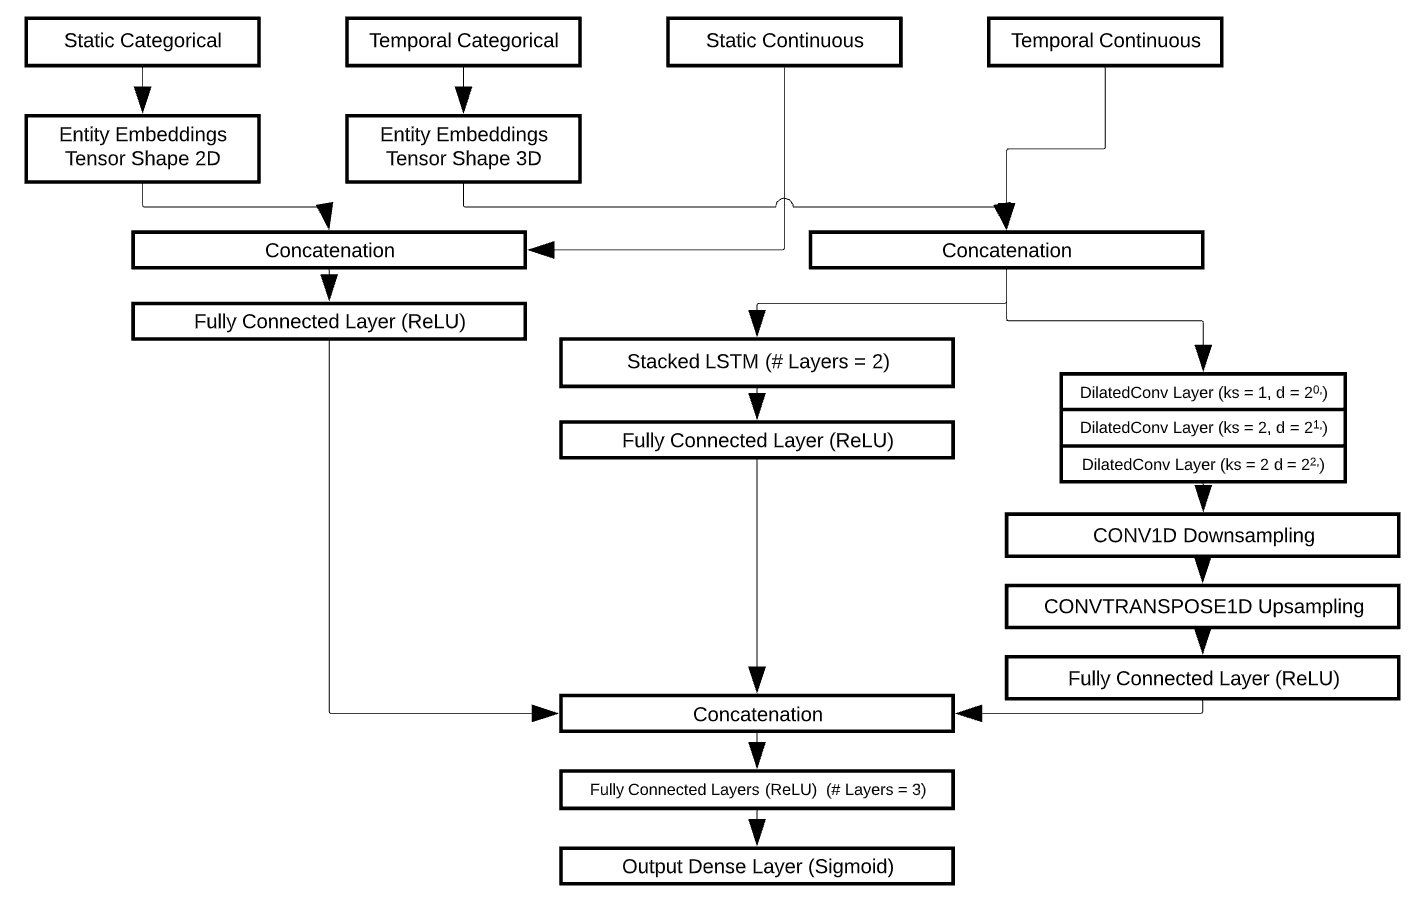
\includegraphics[width=3.3in]{img/TCNLSTM.png} 
    \label{fig:TCN-LSTM} 
  \end{figure}

The consumer purchase pattern has huge variation in terms of time of purchase (weekday/weekends), 
cadence of purchase (days to months), purchased item types (dairy/meat/grocery/apparels/etc.)
and brand loyalty (tendency to substitute items). Given such huge variations, it becomes imperative 
to cross learn consumer behaviour from similar consumer groups. To learn such relationships its 
important to capture non-linear relationship between target and regressors at various levels.
Tree based and Deep learning models are chosen for their ability to model feature interactions (even if transient in time), 
and their ability to capture non-linearity well.

Tree based models and MLP training uses lagged values of time varying regressors
to capture temporal dependencies. LSTM, TCN and TCN-LSTM models are trained using entire life-cycle data of a 
time series (Consumer-Item) in sequential manner. Details around dataset and features are explained in section \ref{sec:eval}. 

\subsection{Hyperparameter Tuning}
Hyper-parameters of tree based models are optimized
using Bayesian Hyperparameter Optimization Technique, Hyperopt \cite{bergstra2013hyperopt}. 
For deep learning, we use documented best practices along with our experimental results to
choose model hyperparameters. Hyperparameter Optimization is performed over Validation dataset. 
We list some of the hyperparameters along with the values we tune for Deep learning models.
  \begin{itemize}
    \item {\bf Optimizer Parameters:} RMSProp \cite{bengio2015rmsprop} and Adam were used as different trial configurations. The learning rate 
    was experimentally tuned to 1e-3. We also did weight decay of 1e-5 which helped a bit in model Regularization.
    \item {\bf Scheduler Parameters:} Cyclic \cite{smith2017cyclical} and ReduceLROnPlateau \cite{zaheer2018adaptive} 
    Learning rates were used as different trial configurations.
    we used 1e-3 as max lr and 1e-6 as base lr for Cyclical learning rate along with the step size being the function of
    length of train loader. ReduceLROnPlateau was tuned for 1e-6 as min lr.
    \item {\bf SWA:} Stochastic Weight Averaging (SWA) \cite{izmailov2018averaging} is used to improve generalization across Deep Learning
    models. SWA performs an equal average of the weights traversed by SGD with a modified learning rate schedule. We used 
    1e-3 as SWA learning rate.
    \item {\bf Parameter Average:} This is another generalization technique, which is weighted average of parameter weights 
    of n minimas post training completion. Weights are based on total val loss for epoch with n set as 2 for our 
    experiments.
  \end{itemize}
Apart from the above parameters we also iterate to tune network parameters like number of epochs, batch size, 
number of Fully Connected Layers, number of LSTM layers, convnet parameters (kernel size, dilations, padding)
and embedding sizes for the categorical features. Binary Cross-Entropy \ref{eqn:logloss} is used as loss 
function for all the models. For sequence model \cite{sutskever2014sequence}, we also iterate with
Dropout \cite{hinton2012improving} and BatchNorm \cite{santurkar2018does} within networks.
Hyperparameters used for Machine learning models with Hyperopt \cite{bergstra2013hyperopt} are :
  \begin{itemize}
    \item {\bf Learning Rate:} Range set to vary between 1e-2 to 5e-1. 
    \item {\bf Max Depth:} Range set from 2 to 12 at step of 1.
  \end{itemize}
Apart from above hyperparameters, Regularization parameters like Reg Lambda and Min Sample Leaf were also optimized using Hyperopt.

Deep learning models are built using deep learning framework
PyTorch \cite{paszke2017automatic}, and are trained on GCP instance containing 6 CPUs and a single GPU. 
Scikit-learn \cite{pedregosa2011scikit} is used for Tree
based models like RandomForest and Xgboost \cite{chen2016xgboost}. For Neural Network Architectures, 
we save model weights of the best checkpoint, so that we may access the learned entity embeddings and other
model weights in case of requirement. As described in Table \ref{tab:modelparams}, we build a total of 60 models, 
12 different configurations for each of 4 Deep Learning models and 6 best trials from Hyperopt \cite{bergstra2013hyperopt} 
for each of 2 Machine Learning models.
\subsection{Stacked Generalization Ensemble}
Stacked generalization or Stacking \cite{wolpert1992stacked} is an ensemble method where a new model learns how to best 
combine the predictions from multiple existing models. This is acieved by training an entirely new model using 
contributions from each submodel. 
We use weighted K-best model as Stacker for combining k submodels (candidates) out of total 60 
trained models. We iterate with different values of k ranging from 3 to 25 as presented in Table \ref{tab:stacking} . 
Test1 BCELoss of submodels is used for weight initialization for the stacker models. For learning optimal weights of submodels, 
we minimise Test1 BCELoss of the stacker model using gradient descent \cite{ruder2016overview}, 
stacking function can be described as:
  \begin{equation}
    \begin{array}{l}
      y\textsubscript{cit} =\sum_{j=1}^{k}w\textsubscript{j} \times p\textsubscript{cit\textsubscript{j}}
    \end{array}
    \label{eqn:stack}
  \end{equation}
where y\textsubscript{cit} is the stacked probability for consumer 'c' for item ’i’ at time ’t’.
k represents the number of candidates shortlisted for stacking, p\textsubscript{cit\textsubscript{j}}
represents the prediction probability for consumer 'c' for item ’i’ at time ’t’ by j\textsuperscript{th} submodel.
w\textsubscript{j} is the weight for j\textsuperscript{th} submodel.

\subsection{F\textsubscript{1}-Maximization}
Post stacking, we optimize for purchase probability threshold based on
probability distribution at a consumer level using F\textsubscript{1}-Maximization.
This enables optimal thresholding of consumer level probabilities to  maximize F\textsubscript{1} measure \cite{lipton2014optimal}.
To illustrate the above, let's say we generated purchase probabilities for 
'n' items out of 'b' actually purchased items by consumer 'c'. Now, lets visualize the actuals (\ref{eqn:A}) 
and predictions (\ref{eqn:P})  of 'n' predicted items for consumer 'c'.
  \begin{equation}
    \begin{array}{l}
      A\textsubscript{c} = [a\textsubscript{1}, a\textsubscript{2}, .., a\textsubscript{n}] 
       \; \forall \; a\textsubscript{j} \in \; $\{0,1\}$
    \end{array}
    \label{eqn:A}
  \end{equation}
  \begin{equation}
    \begin{array}{l}
      P\textsubscript{c} = [p\textsubscript{1}, p\textsubscript{2}, .., p\textsubscript{n}]
      \; \forall \; p\textsubscript{j} \in \; [0,1]
    \end{array}
    \label{eqn:P}
  \end{equation}
A\textsubscript{c} represents the actuals for consumer 'c', with a\textsubscript{j} being 1/0 
(purchased/non purchased). P\textsubscript{c} represents the predictions 
for consumer 'c' for the respective item, with p\textsubscript{j} being probability value. 
'n' is the total items model generated purchase probabilities for consumer 'c'.
Now we apply Decision rule D() which converts probabilities to binary predictions, as described below 
in Equation \ref{eqn:Decision}.
  \begin{equation}
    \begin{array}{l}
      D(Pr\textsubscript{c}) : P\textsubscript{c}\textsuperscript{1 x n}
      \to P\textsuperscript{'}\textsubscript{c}\textsuperscript{1 x n}
      \;\; : p\textsuperscript{'}\textsubscript{j} = 
        \begin{cases}
          1 & p\textsubscript{j} \geq Pr\textsubscript{c} \\
          0 & \text{Otherwise}
        \end{cases}
    \end{array}
    \label{eqn:Decision}
  \end{equation}
  \begin{equation}
    \begin{array}{l}
      P\textsuperscript{'}\textsubscript{c} = [p\textsuperscript{'}\textsubscript{1}, 
      p\textsuperscript{'}\textsubscript{2}, .., p\textsuperscript{'}\textsubscript{n}]\; 
      \forall \; p\textsuperscript{'}\textsubscript{j} \in \; $\{0,1\}$
    \end{array}
    \label{eqn:Pdash}
  \end{equation}
  \begin{equation}
    \begin{array}{l}
      k =\sum_{i=1}^{n}p\textsuperscript{'}\textsubscript{i}
    \end{array}
    \label{eqn:Pdash}
  \end{equation}
Pr\textsubscript{c} is the probability cut-off to be optimized for maximizing F\textsubscript{1} measure \cite{lipton2014optimal} 
for consumer 'c'. Decision rule D() converts probabilities P\textsubscript{c} to binary predictions 
P\textsuperscript{'}\textsubscript{c} such that if p\textsubscript{j} is less than 
Pr\textsubscript{c} then p\textsuperscript{'}\textsubscript{j} equals 0, otherwise 1.
'k' is the sum of predictions generated post applying Decision rule D(). Now we solve for F\textsubscript{1} measure
using equations and formulae described below.
  \begin{equation}
    \begin{array}{l}
      V\textsubscript{Pr\textsubscript{c}} = 
      P\textsuperscript{'}\textsubscript{c}
      \;\times\; A\textsubscript{c}\textsuperscript{T}
      \;
      \Rightarrow	
      \left( \begin{array}{ccc}
      p\textsuperscript{'}\textsubscript{1} & .. & 
      p\textsuperscript{'}\textsubscript{n}
      \end{array} \right)
      \times
      %
      \left( \begin{array}{ccc}
      a\textsubscript{1} \\
      .. \\
      a\textsubscript{n} \\
      \end{array} \right)
    \end{array}
    \label{eqn:probability}
  \end{equation}
  \begin{equation}
    \begin{array}{l}
      Precision\textsubscript{c}= \frac{V\textsubscript{Pr\textsubscript{c}}} {k}
      \;\;\;\;\;and\;\;\;\;
      Recall\textsubscript{c}= \frac{V\textsubscript{Pr\textsubscript{c}}} {b}
    \end{array}
    \label{eqn:F1}
  \end{equation}
  \begin{equation}
    \begin{array}{l}
      F\textsubscript{1\textsubscript{c}} = \frac{2 \times Precision\textsubscript{c} 
      \times Recall\textsubscript{c}} 
      {Precision\textsubscript{c} + Recall\textsubscript{c}}
      \;
      \;\;\;\;\Rightarrow	\;\;\;\;
      2 * 
      \frac{
        V\textsubscript{Pr\textsubscript{c}}
      }
      {
        k + b
      }
    \end{array}
    \label{eqn:Optimizer}
  \end{equation}
V\textsubscript{Pr\textsubscript{c}} represents the number of items with purchase 
probabilities greater than Pr\textsubscript{c} which were actually purchased (True Positives). 
As can be seen, Formulae \ref{eqn:F1} and \ref{eqn:Optimizer} are used to calculate Precision, Recall and 
F\textsubscript{1}-score for consumer 'c'. 

  \begin{equation}
    \max_{V\textsubscript{Pr\textsubscript{c}}} \;\;\;\; 2 * \frac{ V\textsubscript{Pr\textsubscript{c}}}{k + b}
    \;\;\;\;,\;\;\;\;  \text{subject to: } \;\;\;\;  Pr\textsubscript{c}  \in \; [0,1]
    \label{eq:constraint}
  \end{equation}
Equation \ref{eq:constraint} represents the optimization function we use to generate final predictions for each consumer.
\begin{center}
\begin{table*}[!t]
\caption{Model Specifications}
\centering
\resizebox{\textwidth}{!}{\begin{tabular}{|r|l|r|r|}
  \hline
 {\bf Model Type} & {\bf Trials} & {\bf Model HyperParameters} & {\bf Loss Functions}\\ 
 \hline\hline
MLP	  		&  12 & Optimizer, Scheduler, SWA, Parameter Averaging, Feature Groups, FC Layers & BCELoss\\ \hline
LSTM  		& 12 & Optimizer, Scheduler, SWA, Parameter Averaging, Feature Groups, FC Layers, LSTM Layers & BCELoss \\ \hline
TCN			& 12	& Optimizer, Scheduler, SWA, Parameter Averaging, Feature Groups, FC Layers, Convolution Parameters  & BCELoss\\ \hline
TCN-LSTM 		& 12	& Optimizer, Scheduler, SWA, Parameter Averaging, Feature Groups, FC Layers, LSTM, Convolution Parameters  & BCELoss\\ \hline
Xgboost 		& 6	& Learning rate, Tree Depth, Regularization parameters  & BCELoss\\ \hline
RandomForest 		& 6	& Tree Depth, Evaluation Metrics, Regularization parameters &  BCELoss\\
   \hline
\end{tabular}}
\label{tab:modelparams}
\end{table*} 
\end{center}
